\documentclass{article}
% T1 selects the template's Type-1 Times fonts under both pdfLaTeX and Tectonic.
\usepackage[T1]{fontenc}
\usepackage{microtype}
\usepackage{graphicx}
\usepackage{booktabs}
\usepackage{hyperref}
\newcommand{\theHalgorithm}{\arabic{algorithm}}
% User-supplied ICML 2026 template. This is a working draft, not a 2026 submission.
\usepackage{icml2026}
% [noticehidden] working draft: suppress the anonymous-affiliation footnote and the
% "Preliminary work ..." notice. Restore by deleting this redefinition before submission.
\makeatletter
\renewcommand{\printAffiliationsAndNotice}[1]{\global\icml@noticeprintedtrue}
\renewcommand{\@pa}[1]{}  % drop the dangling affiliation superscript in the hidden-footnote draft
\makeatother
\usepackage{amsmath,amssymb,mathtools}
\usepackage{tikz}
\usetikzlibrary{arrows.meta,positioning}
\newcommand{\method}{MPCache}
\newcommand{\R}{\mathbb{R}}
\newcommand{\norm}[1]{\left\lVert #1 \right\rVert}
\newcommand{\E}{\mathbb{E}}
\newcommand{\eps}{\varepsilon}
\icmltitlerunning{MPCache: Model-Predictive Caching}
\begin{document}
\twocolumn[
\icmltitle{MPCache: Model-Predictive Caching for\\ Training-Free Video Diffusion Acceleration}
\begin{icmlauthorlist}
\icmlauthor{Anonymous Authors}{}
\end{icmlauthorlist}
% Anonymous affiliation block hidden for the working draft; restore for submission:
% \icmlaffiliation{anon}{Anonymous Institution}
% \icmlcorrespondingauthor{Anonymous Author}{anonymous@example.invalid}
\icmlkeywords{Diffusion Transformers, Training-Free Acceleration, Feature Caching, Model Predictive Control}
\vskip 0.3in
]
\printAffiliationsAndNotice{}
\begin{abstract}
Video diffusion transformers are costly to sample: every step runs the denoiser twice under classifier-free guidance. Training-free caching replaces some evaluations with cached features or cheap forecasts, but chooses when to skip and what to return with separate rules, so a cheap-looking skip can still return a value whose error later steps amplify. Inspired by model-predictive control, we propose \method, which identifies one small model of the denoising dynamics online, at zero extra denoiser calls, and uses it three ways: State-Conditioned Forecasting predicts skipped steps from the current latent, Solver-Aware Pricing propagates the forecast error to the terminal step, and a Residual Check updates the model and its trust region at every exact evaluation. A receding-horizon planner then allocates the evaluation budget across the trajectory. A skip now carries an explicit cost before it is taken rather than being discovered after. Weights and sampling grids are untouched. Experiments on CogVideoX-2B and Wan2.1-T2V-1.3B demonstrate improved efficiency--fidelity trade-offs over TeaCache, TaylorSeer, and RA-CFGCache at matched exact-evaluation budgets. Code is available at \url{https://github.com/Yizhou-Yang/MPCache}.
% CLAIM PENDING (2026-10-20): the empirical sentence above is a TARGET, not a measured result.
% Gate before submission: matched-budget median reduction >= 25%, win rate >= 0.75, effect > 2 SEM,
% on both backbones, with the table it points to filled in. Until then this draft must not be submitted.
% ANONYMITY: for submission replace the URL with an anonymous mirror (e.g. anonymous.4open.science).

\end{abstract}
\section{Introduction}
Diffusion transformers have become important backbones for image and video generation \citep{peebles2023dit,yang2025cogvideox,wan2025wan}. Their inference cost is dominated by repeated denoiser evaluations over a sampling trajectory, with long video token sequences making each evaluation expensive. Training-free caching offers an attractive alternative to retraining: retain the pretrained network and sampling schedule, but replace some expensive computations with previously cached quantities or inexpensive predictions. Two decisions govern the resulting quality--efficiency trade-off: \emph{what should a skipped computation return, and when is that approximation worth its downstream cost?}

Existing methods address complementary parts of this problem. TeaCache uses changes in timestep-modulated inputs as inexpensive proxies for output variation and controls reuse with a rescaled, accumulated signal \citep{liu2025teacache}. TaylorSeer forecasts intermediate features from finite-difference estimates of temporal derivatives \citep{liu2025taylorseer}. RA-CFGCache aligns cache decisions with classifier-free guidance (CFG) and rescales local guided-risk estimates using an offline-calibrated, timestep-dependent propagation prior \citep{liu2026racfgcache}. These approaches are not simply equivalent to treating the denoiser as a time series: TeaCache already observes input-dependent signals, and RA-CFGCache explicitly accounts for downstream propagation. The remaining question is whether a \emph{causal, per-trajectory dynamics model} can improve both the approximation itself and the choice of where to spend exact computation.

The distinction matters because forecasting and scheduling interact through the latent state. Write a guided denoiser as $v_i=f(x_i,\tau_i)$, where $x_i$ is the current latent and $\tau_i$ the scheduler's noise coordinate. A temporal forecaster estimates changes along the trajectory represented by its cached observations. Once a prediction is used, however, the sampler evolves to a different latent; the next prediction is queried on this altered trajectory. Similarly, two forecast errors of equal magnitude can have different downstream effects because the solver and denoising field transform their directions differently. A scheduling rule cannot generally evaluate one forecast independently of the states and cache anchors induced by earlier choices. This motivates joint selection, not a claim that local proxies are always inferior.

\method\ addresses this coupling by caching a local model rather than only an output. At exact evaluation points, it records latent--output pairs and fits a channel-diagonal plus low-rank affine approximation to the guided field. At skipped steps, the current latent is already available from the sampler and can be used directly in that approximation. The fitted operator also defines a local tangent model of the sampling update, yielding a surrogate for the propagation of forecast error. The controller uses that surrogate to compare compute, reuse, temporal extrapolation, and state-conditioned prediction under a remaining evaluation budget. When a new exact evaluation arrives, its pre-update prediction residual tests the model, tightens or relaxes the trust region, and triggers replanning. Thus forecasting, pricing, and feedback refer to the same identified object rather than three independently calibrated components.

This is a discrete-action instance of model predictive control: identify a model from available observations, predict the consequences of candidate actions, execute one action, and repeat \citep{rawlings2017mpc}. The analogy is operational, not a transfer of classical MPC stability guarantees. A denoising trajectory provides limited excitation; its time drift and state response can be confounded. A model that predicts outputs along that trajectory may still misrepresent the off-trajectory directions needed for error propagation. Our initial channelwise finite-difference diagnostic did not establish useful propagation pricing. We therefore treat propagation fidelity as an empirical gate, not as an already demonstrated consequence of caching a local model. The proposed structured, causal estimator and the full controller remain to be validated.

The intended methodological contributions are:
\begin{itemize}
\item \textbf{One model for two coupled decisions.} A regularized local guided-field model is shared by state-conditioned forecasting and solver-aware cost estimation, with explicit limits on what trajectory observations can identify.
\item \textbf{Budgeted receding-horizon cache control.} A controller jointly selects refresh times and prediction operators while retaining scheduler and cache-history state; approximate search is distinguished from exact dynamic programming.
\item \textbf{Residual-based model checking.} Exact evaluations provide causal, pre-update diagnostics that govern trust and replanning without additional probe evaluations.
\end{itemize}
These are design contributions in the present draft, not claims of verified performance. The evaluation target is a common protocol on CogVideoX-2B and Wan2.1-T2V-1.3B against TeaCache, TaylorSeer, and RA-CFGCache, with matched budgets, paired fidelity measurements, and separately measured runtime overhead. A successful result must demonstrate that the shared model improves the joint decision, not merely that any one of its components is useful.

\begin{figure*}[t]
\centering
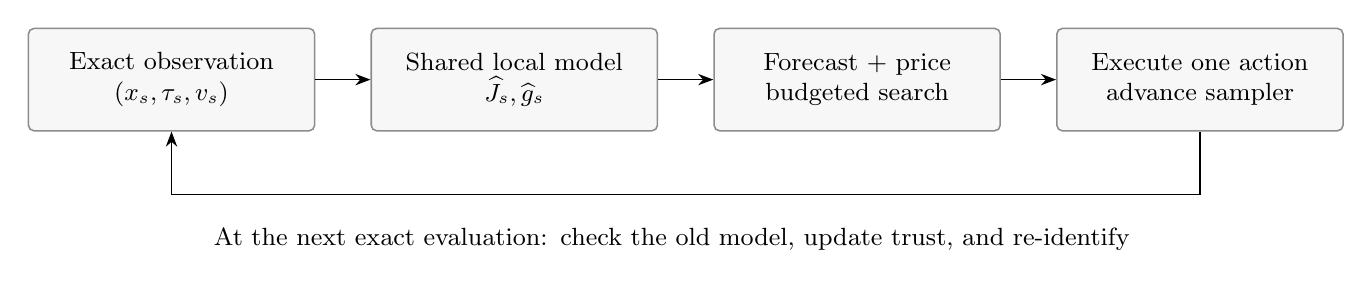
\begin{tikzpicture}[node distance=7mm and 7mm, >=Stealth,
 box/.style={draw=black!45, rounded corners=2pt, fill=black!3, align=center, font=\small, minimum height=13mm, text width=34mm},
 every path/.style={line width=0.55pt}]
\node[box] (observe) {Exact observation\\$(x_s,\tau_s,v_s)$};
\node[box,right=of observe] (identify) {Shared local model\\$\widehat J_s,\widehat g_s$};
\node[box,right=of identify] (plan) {Forecast + price\\budgeted search};
\node[box,right=of plan] (execute) {Execute one action\\advance sampler};
\draw[->] (observe)--(identify);
\draw[->] (identify)--(plan);
\draw[->] (plan)--(execute);
\draw[->] (execute.south)--++(0,-8mm)-| (observe.south);
\node[below=11mm of identify.south,xshift=20mm,text width=125mm,font=\small,align=center] {At the next exact evaluation: check the old model, update trust, and re-identify};
\end{tikzpicture}
\caption{\method\ design. A causal local model is shared by forecasting and propagation-aware planning; the feedback observation is an ordinary budgeted evaluation, not an additional probe.}
\label{fig:loop}
\end{figure*}

\section{Related Work}
\paragraph{Training-free reuse and forecasting.}
TeaCache estimates nonuniform output variation from inexpensive, timestep-modulated inputs and rescales the estimated changes for adaptive caching \citep{liu2025teacache}. Its input sensitivity is important: our distinction is not simply that prior work ignores the current latent. TaylorSeer replaces direct reuse with Taylor-series feature forecasts whose derivatives are approximated from historical feature values \citep{liu2025taylorseer}. \method\ instead proposes an explicit state-and-time model of the guided output. Its temporal fallback is an output-level first-order extrapolator, not a reproduction of TaylorSeer's intermediate-feature implementation. Comparisons must use the actual baseline code and identify any model-specific adaptation.

\paragraph{Guidance- and propagation-aware cache control.}
RA-CFGCache identifies both a branch-guided mismatch and a local-final mismatch under CFG \citep{liu2026racfgcache}. It composes branch-wise error proxies using guidance coefficients and calibrated cross-branch alignment, then applies a timestep-dependent propagation prior before online thresholding. Consequently, propagation-aware caching itself is prior work, not our novelty claim. The proposed distinction is a causal, prompt-specific local operator shared by output prediction and finite-horizon action selection. Whether that operator adds information beyond a timestep prior is unresolved and must be measured; substituting such a prior into \method\ is a necessary ablation, not evidence for online identification.

\paragraph{Numerical sampling.}
DDIM and UniPC reduce the number of denoising evaluations through sampling schemes with different update rules and solver histories \citep{song2021ddim,zhao2023unipc}. \method\ keeps the selected sampling grid and scheduler fixed and changes which steps receive exact network outputs. Its propagation model must therefore use the actual scheduler, including prediction-type conversion and multistep history. A one-step tangent formula is not automatically valid for a predictor--corrector scheduler.

\paragraph{Online identification and predictive control.}
Secant and quasi-Newton methods construct derivative approximations from function evaluations without forming a dense Jacobian \citep{broyden1965class}. We borrow this limited-memory identification principle, but fitting along a denoising trajectory is not equivalent to observing fixed-time state perturbations. Model predictive control repeatedly optimizes a finite-horizon action sequence and executes only its first action \citep{rawlings2017mpc}. \method\ uses that structure for compute allocation; low-rank fitting, receding-horizon planning, and residual checks are not individually claimed as new. The research hypothesis is that coupling them through one useful dynamics model yields a better cache controller.

\paragraph{Video models and evaluation.}
CogVideoX and Wan provide the two video backbones used in the planned comparison \citep{yang2025cogvideox,wan2025wan}. VBench supplies a multidimensional video-evaluation framework \citep{huang2024vbench}. Using its prompt resource for paired LPIPS, SSIM, and PSNR is distinct from computing a full VBench score. We follow RA-CFGCache's shared generation protocol for reproducibility and will report these evaluation scopes separately.

\section{Method: Model-Predictive Caching}
\label{sec:method}
Caching is a trust-region problem. A skipped evaluation is a step taken on the strength of a local model rather than on the true field, so the controller has to decide how large a step the model can be trusted with. Trust-region methods answer exactly this question: build a local model, predict what a step will do, compare the prediction with what actually happens, and expand or shrink the radius accordingly. \method\ applies that loop to caching. The model is fitted online from the exact anchors, the price predicts the terminal effect of a skip, and every exact evaluation is the ratio test that expands or shrinks how far the next skip may reach. Sections~\ref{sec:core}--\ref{sec:control} follow the loop: model, predicted effect, radius.

\subsection{Preliminaries}
\label{sec:prelim}
Consider a fixed prompt, guidance scale $\omega$, and denoising grid $i=0,\ldots,T-1$, with latent $x_i\in\R^d$ and noise coordinate $\tau_i$. At each step the solver consumes the guided output $v_i=f(x_i,\tau_i)=u_i+\omega(c_i-u_i)$, where $u_i$ and $c_i$ are the unconditional and conditional predictions; an exact evaluation computes both branches and costs one unit of the budget $B$. With augmented state $z_i$ holding the latent and any solver history, the solver applies the transition $z_{i+1}=S_i(z_i,\widetilde v_i)$ with $x_i=Pz_i$, where $\widetilde v_i$ is the exact or approximate output; for an affine one-step solver, $x_{i+1}=a_ix_i+b_i\widetilde v_i$. Caching replaces $v_i$ by $\widetilde v_i$ and leaves $S_i$ unchanged. At step $i$ the controller sees only $z_i$ and the causal buffer $\mathcal B_i$ of past exact evaluations, and must decide whether to evaluate or to forecast. Three errors follow: the forecast may misestimate the skip, a small misestimate may grow before the terminal step, and the controller may misjudge when to refresh. Sections~\ref{sec:core}--\ref{sec:control} address them in order.

\paragraph{Standard formulation.} We borrow the learning-based model predictive control formulation of \citet{hewing2021learning}, in which a model fitted from logged transitions is used inside a finite-horizon problem,
\begin{equation}
 \begin{aligned}
 &\min_{\pi=(a_i,\ldots,a_{i+H-1})}\ \sum_{j=i}^{i+H-1}c_j(z_j,a_j)+c_H(z_{i+H})\\
 &\text{s.t.}\quad z_{j+1}=\widehat f\!\left(z_j,a_j;\theta\right),\quad a_j\in\mathcal A,
 \end{aligned}
 \label{eq:mpc}
\end{equation}
with stage cost $c_j$, terminal cost $c_H$, and admissible set $\mathcal A$; the model parameters are obtained by regularized least squares on the transitions seen so far, the standard fit in learning-based control \citep{hewing2021learning},
\begin{equation}
 \theta\leftarrow\arg\min_{\theta}\ \sum_k w_k\norm{v_k-\widehat f(x_k,\tau_k;\theta)}^2+\lambda\norm{\theta}^2 .
 \label{eq:fit}
\end{equation}
The two constructions in Equations~\eqref{eq:mpc}--\eqref{eq:fit} are stated as given; we add no analysis of our own to them.

\subsection{The local model}
\label{sec:core}
A cache needs a model of what a skipped evaluation would have returned. The only samples available are the exact evaluations already made, so the model is identified from those anchors at no extra network call. One trajectory visits only a narrow part of the latent space, and the parameterization below is chosen so that this part is what gets identified.

\paragraph{Model.} Around the most recent exact anchor $s$ the guided field is locally linear, so a small change in the latent produces a proportional change in the output. Writing the output as a function of the latent, $v(x)\approx v_s+A(x-x_s)$. The latent also drifts with the noise coordinate, so we compare against straight-line prediction and keep only the part of the change that the line does not explain,
\begin{equation}
 m=u+A\,e,
 \qquad
 e=(x-x_s)-r\,(x_s-x_{s'}),
 \label{eq:model}
\end{equation}
with $u=v_s+r(v_s-v_{s'})$ and $r=(\tau-\tau_s)/(\tau_s-\tau_{s'})$. Here $e$ is the residual motion: the part of $x-x_s$ that straight-line motion does not explain. With $A=0$ the model is plain temporal extrapolation. A full matrix is too large for video latents, so $A$ is a diagonal scaling plus a rank-$r$ correction over recent latent differences, at $O(dr)$ cost. We fit $A$ on differences between anchors by weighted least squares, regularized toward zero, so the model falls back to extrapolation when the residual motion is weak.

\paragraph{The step and its prediction.} A skip returns the anchor $v_s$, the extrapolation $u$, or the model prediction
\begin{equation}
 v=u+w\,(m-u),
 \qquad w\in[0,1],
 \label{eq:forecast}
\end{equation}
where $w$ is a confidence that rises when $m$ beats $u$ at exact checks and halves otherwise. It is the only scalar the controller tunes online: $w=1$ trusts the model, $w=0$ trusts extrapolation. A skip is admissible only while the anchor distance and the anchor age stay inside their trust radii.

\paragraph{Radius.} Each skip carries the cost $c=\|v-m\|+q$, where $q$ is an uncertainty that increases with the distance and age of the anchor, so a skip that reaches further from its anchor pays more even when its nominal error is small.

\subsection{Pricing: the predicted effect of a step}
\label{sec:price}
A local error is not a terminal error. The solver multiplies each output error by its own sensitivity and carries it forward, so the same local error can be harmless at one step and decisive at another. Rather than forming that product, we accumulate a risk $C\leftarrow\alpha C+\beta c$ along each candidate action sequence, with factors estimated from the model; an exact action adds nothing and only carries $C$ forward.

\subsection{Control: trust region under a budget}
\label{sec:control}
With a forecast and a price, the remaining question is where to spend exact evaluations. With remaining budget $b_i$ and horizon $H$, the controller minimizes the accumulated risk subject to a budget that reserves tail refreshes,
\begin{equation}
 \min_{\pi}\ C(\pi)\quad\text{s.t.}\quad
 \sum_{j=i}^{i+H-1}\mathbf 1[a_j=\mathsf C]\le b_i-b_{\rm tail},
 \label{eq:plan}
\end{equation}
over trust-admissible actions. Rollouts use $m$ as the nominal transition and do not call the denoiser. A beam search keeps the top $K$ partial sequences, executes only the first action, and replans, so a misestimate changes the next decision rather than committing the controller.

\paragraph{Residual check.} Every exact evaluation also tests the model. Before refitting, we compare the value the model predicted for that step, $m$, with the value actually computed, $v_s$, and record the relative error
\begin{equation}
 \mathrm{err}=\frac{\|v_s-m\|}{\|v_s\|}.
 \label{eq:check}
\end{equation}
If $\mathrm{err}$ exceeds the current uncertainty $q$, the controller tightens the trust radii and shortens the maximum gap; after consecutive checks inside the envelope it relaxes them. The new anchor is appended, the model refitted, and planning restarts at the next step. The update costs $O(dr)$ and the search is over surrogate transitions, so no extra network call is made.

\section{Experiments}
\label{sec:experiments}
\paragraph{Models, prompts, and fidelity.}
We adopt the protocol of RA-CFGCache Table~1 \citep{liu2026racfgcache} so that our numbers can be placed next to the three closest training-free baselines without re-tuning them. CogVideoX-2B \citep{yang2025cogvideox} generates 49 frames at $720\times480$ and 8\,fps with 50 sampling steps and guidance scale 6. Wan2.1-T2V-1.3B \citep{wan2025wan} generates 81 frames at $832\times480$ and 16\,fps with 50 UniPC steps \citep{zhao2023unipc}, flow shift 3, and guidance scale 5. Prompts are the non-empty lines of the VBench prompt resource \citep{huang2024vbench} used by that harness, of which there are 100; prompt $k$ uses seed $k$, negative prompt ``animation'', and batch size one. Every accelerated video is compared with the full 50-step video of the same prompt and seed by LPIPS (AlexNet), SSIM, and PSNR. Using the VBench prompt list does not constitute a VBench evaluation; reference-free VBench dimensions are reported separately when they are run.

\paragraph{Baselines.}
TeaCache \citep{liu2025teacache} uses thresholds 0.2 (CogVideoX) and 0.15 (Wan); TaylorSeer \citep{liu2025taylorseer} uses interval 3, order 1, and three warm-up steps; RA-CFGCache-Slow/Fast use thresholds 0.6/1.4 (CogVideoX) and 0.4/0.6 (Wan) with the released calibration tables. All baselines run inside the pinned public RA-CFGCache harness, which also contains the TeaCache and TaylorSeer implementations, with two corrections that do not change any method. First, the pinned sampling script forwarded the command-line threshold under a key that the RA-CFGCache controller does not read, so both nominal variants silently ran at the default threshold; we bind the threshold explicitly and assert the effective value at run time. Second, all denoising and caching run on the GPU without CPU offload.

\paragraph{Hardware deviations.}
The published numbers use an H200 in bf16. We run the identical protocol on four H20-96GB cards in bf16, with no CPU offload, no VAE tiling, and no text-encoder parking, so the precision matches the paper and the only deviation is the accelerator itself. A single V100-32GB in fp16 was used as a cross-check: it reproduces CogVideoX and the four Wan rows at $n{=}32$, but its 31.7\,GiB cannot hold TaylorSeer's per-layer derivative cache on Wan, which needs roughly 90\,GiB across the two CFG branches. Latencies are chunk averages measured while four cards are busy, so they are provisional; the quality columns are the comparable ones. All wall-clock numbers for the controller, including its online-identification overhead, will be re-timed on an otherwise idle device.

\begin{table*}[t]
\centering
\small
\setlength{\tabcolsep}{4.2pt}
\caption{Paired 100-prompt baseline reproduction on CogVideoX-2B and Wan2.1-T2V-1.3B (ours: H20-96GB \texttt{bfloat16}; paper: published H200 \texttt{bfloat16} values from \citet{liu2026racfgcache}). RA-CFGCache-Slow achieves the strongest reconstruction fidelity across both backbones; $^\dagger$speedup ratios reflect different GPU architectures.}
\label{tab:baselines}
\begin{tabular}{llccccc}
\toprule
Model & Method & $n$ & LPIPS$\downarrow$ & SSIM$\uparrow$ & PSNR$\uparrow$ & Speedup$^\dagger$ \\
 & & & ours / paper & ours / paper & ours / paper & ours / paper \\
\midrule
CogVideoX-2B & Full ($T{=}50$) & 100 & 0.0000 / 0.0000 & 1.0000 / 1.0000 & $\infty$ / $\infty$ & 1.00$\times$ / 1.00$\times$ \\
 & Fewer steps ($T{=}25$) & 100 & 0.4704 / 0.4751 & 0.5350 / 0.5445 & 14.08 / 13.61 & 1.89$\times$ / 1.86$\times$ \\
 & TeaCache & 100 & 0.2122 / 0.2040 & 0.7392 / 0.7538 & 21.22 / 21.48 & 2.64$\times$ / 2.42$\times$ \\
 & TaylorSeer ($N{=}3,O{=}1$) & 100 & 0.4047 / -- & 0.5626 / -- & 15.38 / -- & 2.36$\times$ / -- \\
 & RA-CFGCache-Slow & 100 & 0.0990 / 0.0968 & 0.8661 / 0.8746 & 26.89 / 26.93 & 2.63$\times$ / 2.39$\times$ \\
 & RA-CFGCache-Fast & 100 & 0.2092 / 0.2052 & 0.7493 / 0.7614 & 21.88 / 21.89 & 3.74$\times$ / 3.13$\times$ \\
\midrule
Wan2.1-T2V-1.3B & Full ($T{=}50$) & 100 & 0.0000 / 0.0000 & 1.0000 / 1.0000 & $\infty$ / $\infty$ & 1.00$\times$ / 1.00$\times$ \\
 & Fewer steps ($T{=}25$) & 100 & 0.4204 / 0.4371 & 0.5700 / 0.5658 & 15.85 / 15.87 & 1.96$\times$ / 1.93$\times$ \\
 & TeaCache & 100 & 0.1681 / 0.1661 & 0.7887 / 0.7955 & 22.84 / 23.08 & 2.53$\times$ / 2.44$\times$ \\
 & TaylorSeer ($N{=}3,O{=}1$) & 100 & 0.3496 / 0.3632 & 0.6283 / 0.6187 & 17.10 / 16.96 & 2.47$\times$ / 2.13$\times$ \\
 & RA-CFGCache-Slow & 100 & 0.0941 / 0.0993 & 0.8820 / 0.8778 & 28.11 / 28.03 & 2.65$\times$ / 2.56$\times$ \\
 & RA-CFGCache-Fast & 100 & 0.1352 / 0.1409 & 0.8420 / 0.8386 & 26.14 / 26.12 & 3.14$\times$ / 2.99$\times$ \\
\bottomrule
\end{tabular}
\end{table*}


\paragraph{Reproduced baselines.}
Table~\ref{tab:baselines} reports all 100 prompts of both backbones; every row has 100 paired samples and no row is imputed. Across the five rows that the published table also contains, LPIPS differs by at most 0.017, SSIM by at most 0.015 and PSNR by at most 0.5\,dB, and the ordering is identical: RA-CFGCache-Slow is the strongest fidelity baseline on both models, TeaCache and RA-CFGCache-Fast trade places with the backbone, and 25 steps is the weakest non-trivial row. This makes RA-CFGCache-Slow the primary comparison for any matched-budget claim. The speedups are not comparable to the published ones: they are chunk averages on four busy H20 cards, and H20 is not H200. TaylorSeer on Wan is reproduced here for the first time in this project ($0.3496$ LPIPS at $2.47\times$); it is clearly worse than TeaCache at a comparable budget, the same pattern as the published Wan row, so its poor CogVideoX result is a property of the method's first-order time extrapolation and not an implementation error. One prompt (id 56 on CogVideoX) collapses to a white clip for the reference and for every method; excluding it moves the row means by at most 0.004 LPIPS and changes no ordering. No statistical gate is claimed for the baselines.

\paragraph{Development platform and component gates.}
Components of \method\ are first tested on a cheaper development setting: CogVideoX-2B, 17 frames at $720\times480$, 30 DDIM steps \citep{song2021ddim}, guidance 6, and eight fixed prompts with two seeds each (16 paired samples). These prompts are disjoint from the evaluation prompts. Each component must pass a pre-registered gate before it enters the full controller. For the forecaster, all methods compute exactly the same steps, given by the static TeaCache schedule at $N\in\{10,13,17\}$ exact evaluations, and differ only in what skipped steps return. Fidelity is the relative $\ell_2$ error of the terminal latent against the all-exact run. The forecaster passes if no sample diverges and the paired median error decreases by at least 10\% relative to the better of reuse and first-order temporal extrapolation at every budget. For propagation pricing, a causal estimate must rank the terminal effect of single-step perturbations better than a leave-one-prompt-out timestep prior of the RA-CFGCache type. The full controller is then compared at matched exact-evaluation budgets with the same forecasts under fixed and prior-based schedules, with paired tests requiring at least 16 samples, a median improvement of at least 25\%, a win rate of at least 0.75, and an effect larger than twice its standard error.

\paragraph{Limitations.}
\textbf{\method\ has no validated result.} Both pre-registered component gates fail: the online propagation price ranks terminal error at Spearman $0.33$ against $0.95$ for a timestep prior, and the state-conditioned forecaster beats the better of reuse and first-order extrapolation by $9.1\%$ at $N{=}13$ but loses $22\%$ at $N{=}10$. The controller has therefore never been run end-to-end at the scale of Table~\ref{tab:baselines}, which reports baselines only. The reproduction also runs on four H20 cards rather than the published H200, so only the quality columns are comparable; one CogVideoX prompt collapses to a white clip for the reference and for every method; and each baseline is evaluated at the budget its own scheduler selects, so its wall-clock advantage over a fixed budget is not uniform.


% References start on a fresh page (not required by ICML, but it keeps the page budget
% and the editing boundaries easy to read).
\clearpage
\bibliographystyle{icml2026}
\begingroup
\raggedbottom
\bibliography{references}
\endgroup

% Appendix starts on its own page as well; uncomment when the first appendix section exists.
% \clearpage
% \appendix
% \section{Appendix}

\end{document}
